\section{Results and Discussion}
\label{sec:results}

As discussed in section~\ref{sec:design}, we perform our evaluations on 
binaries found in the GNU Coreutils package as well as the libraries in 
OpenSSL. We built GNU Coreutils and OpenSSL using LLVM 3.4, and also built 
the same binaries with obfuscations using the same compiler. We built 
different versions of the obfuscated binaries, for different types of 
obfuscations supported by Obfuscator-LLVM and discussed in 
section~\ref{sec:obfllvm}, and a binary with all the obfuscations. In our 
discussion, unless otherwise specified, an obfuscated binary refers to a 
binary built with all the supported obfuscations. 

While the OpenSSL libraries libssl.a and libcrypto.a are a collection of 
object files, we need an ELF binary in order to find ROP gadgets. We 
created a small test program and then statically linked the objects from 
both binaries with this program to create a binary which we can use for 
evaluation. We refer to this combined binary of objects from libssl and 
libcrypto as libssl. 

Once we identify gadgets in a binary, we also categorize these gadgets 
based on the instructions they contain and the function they can serve. 
The categories are

\begin{itemize}
    \item Memory: These are instructions and gadgets that facilitate load  
    and store operations from/to memory and registers. 
    \item Arithmetic: These are gadgets that contain arithmetic 
    instructions and which can be used to perform operations such as add, 
    sub, neg, etc. 
    \item Logic: These are gadgets that contain instructions or can be 
    used to perform operations such as and, or, xor, shift, rotate, etc.
    \item Control: These are gadgets that can control the flow, such as 
    conditional or unconditional jumps. 
    \item Other: These are gadgets that we could not categorize.
\end{itemize}


\begin{figure}[h]
    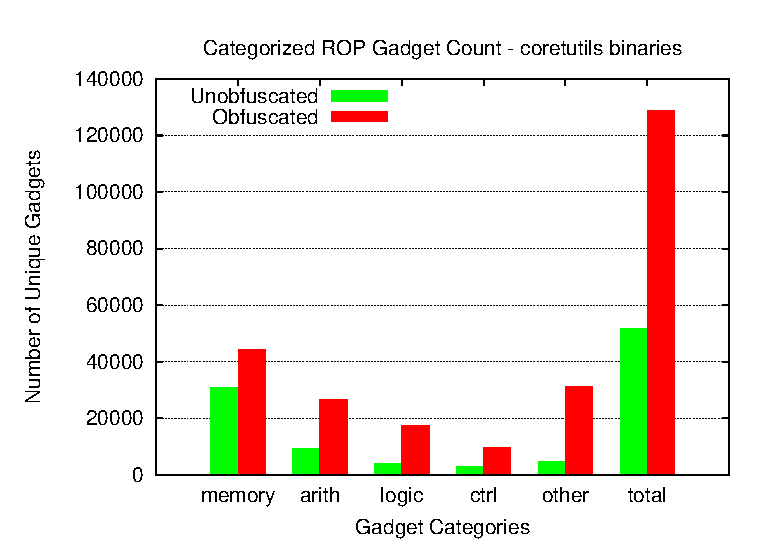
\includegraphics[width=\linewidth]{figures/coretutils-aggregate.eps}
    \captionsetup{font=footnotesize, labelfont=bf, justification=centering}
    \caption{Gadget count for `coreutils' binaries}
    \label{fig:coreutil}
\end{figure}

\begin{figure}[h]
    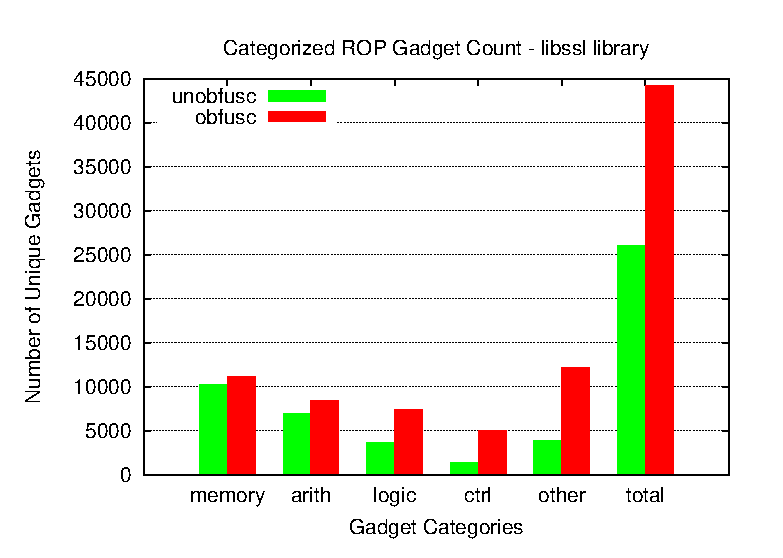
\includegraphics[width=\linewidth]{figures/libssl.eps}
    \captionsetup{font=footnotesize, labelfont=bf, justification=centering}
    \caption{Gadget count for `libssl' library}
    \label{fig:libssl}
\end{figure}

Figure~\ref{fig:coreutil} shows the categorized as well as the total 
gadget counts aggregated for all the binaries in Coreutils with and 
without obfuscation. We can see that obfuscation more than doubles the 
total gadgets in the binaries, however the impact varies across 
categories. Similar graph for libssl is shown in Figure~\ref{fig:libssl}, 
where the total increase is more moderate. We believe this was because the 
obfuscator we are using was not able to handle some of the more 
complicated and large source files in libssl, and hence abandoned 
obfuscations on them. However, both these graphs show that obfuscation 
significantly increases the number of gadgets in a binary.

\subsection{Impact of Obfuscation Type}
% talk about different types of obfusc and their impact

\begin{table} [h]
    \centering
    \begin{adjustbox}{max width=\linewidth}
    \begin{tabular}{|l|r|r|r|r|r|}
        \hline
        \bf Binaries & \bf unobfusc & \bf sub-obfusc & \bf bcf-obfusc & \bf fla-obfusc & \bf all-obfusc \\
        \hline
        \bf link & 44 & 48 & 81 & 92 & 149 \\
        \bf chroot & 59 & 59 & 111 & 131 & 223 \\
        \bf shred & 85 & 97 & 169 & 185 & 313 \\
        \bf date & 101 & 113 & 217 & 277 & 473 \\
        \bf cp & 169 & 185 & 381 & 425 & 757 \\
        \bf coreutils & 11264 & 9318 & 17408 & 20480 & 41984 \\
        \hline
    \end{tabular}
    \end{adjustbox}
    \captionsetup{font=footnotesize, labelfont=bf, justification=centering}
    \caption{Binaries size (in KBs) with different obfuscation techniques}
    \label{tab:binsize}
\end{table}

Table \ref{tab:binsize} shows the binary sizes for some of the utilities 
in GNU Coreutils along with their size with different obfuscations. The 
instruction substitution obfuscation is referred to as sub-obfusc (or 
SUB), bogus control flow as bcf-obfusc (or BCF) and control flow 
flattening as fla-obfusc (or FLA), and details of these obfuscations are 
discussed in section~\ref{sec:obfllvm}. As expected, substitution does not 
have as big an impact on binary size as the other two. The size increases 
in binaries with full obfuscation ranged from about 3x to 5x. 

\begin{table} [htbp]
    \centering
    \begin{adjustbox}{max width=\linewidth}
    \begin{tabular}{|c|c|c|c|c|}
        \hline
        \bf Categories & \bf sub-obfusc & \bf bcf-obfusc & \bf fla-obfusc & \bf all-obfusc \\
        \hline
        \bf memory & 4.70 & 17.80 & 12.87 & 43.86	\\
        \bf arith & 32.16 & 180.85 & 137.09 & 189.01 \\
        \bf logic & 56.82 & 85.52 & 112.43 & 352.41 \\
        \bf ctrl & 19.12 & 85.73 & 111.81 & 219.62 \\ 
        \bf other & 98.96 & 117.09 & 258.99 & 552.37 \\
        \bf total & 23.08 & 65.20 & 71.11 & 150.16 \\
        \hline
    \end{tabular}
    \end{adjustbox}
    \captionsetup{font=footnotesize, labelfont=bf, justification=centering}
    \caption{Increase in gadgets found in Coreutils as a percentage of gadgets in unobfuscated binaries}
    \label{tab:gadget_increase}
\end{table}

\begin{figure}
    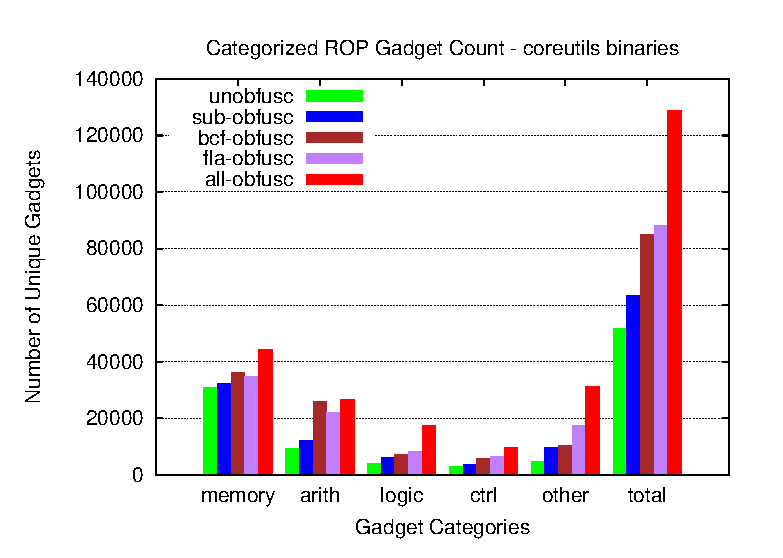
\includegraphics[width=\linewidth]{figures/coretutils-aggregate-all.eps}
    \captionsetup{font=footnotesize, labelfont=bf, justification=centering}
    \caption{Different types of obfuscation for all `coreutils' binaries}
    \label{fig:types_of_obfusc}
\end{figure}

The impact of different obfuscation types on gadgets is shown in 
Figure~\ref{fig:types_of_obfusc}. It is clear that while overall the 
impact of BCF and FLA are higher than SUB, their impact within specific 
categories of gadets varies. The percentage increase for different types 
of obfuscations across categories is shown in 
Table~\ref{tab:gadget_increase}. Since aggregating across all of Coreutils 
binaries is difficult to analyze, we do more detailed analysis on a few 
selected binaries in Coreutils as identified in 
section~\ref{sec:sampleselect}. The graphs for \texttt{cp} and 
\texttt{link} are shown in Figures~\ref{fig:cp_all} and  
~\ref{fig:link_all}. We can see that on certain binaries like 
\texttt{link} BCF obfuscation has significantly more gadgets than FLA, but 
overall both types of obfuscation have similar impact on increase in 
gadgets. 

\begin{figure}[h]
    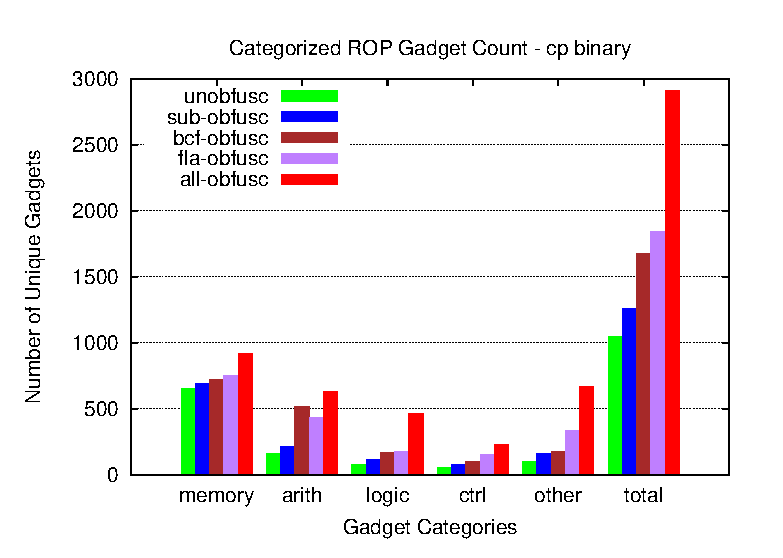
\includegraphics[width=\linewidth]{figures/cp-all.eps}
    \captionsetup{font=footnotesize, labelfont=bf, justification=centering}
    \caption{Different types of obfuscation for `cp' binary}
    \label{fig:cp_all}
\end{figure}


\begin{figure}[h]
    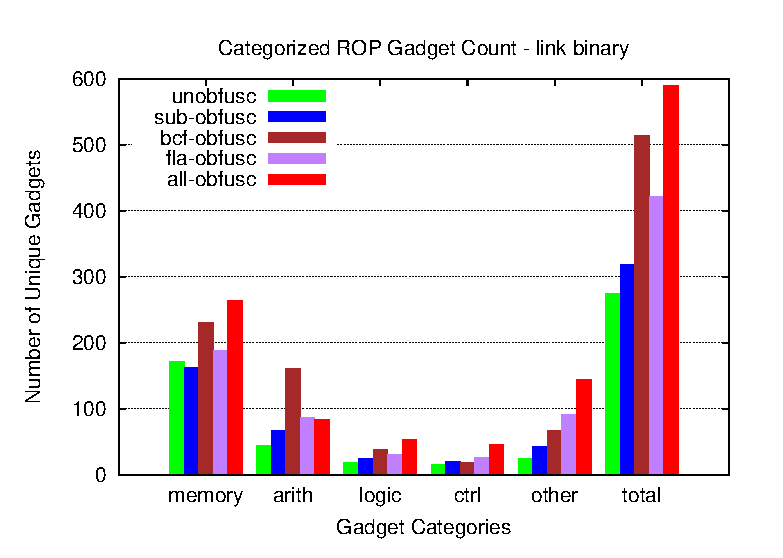
\includegraphics[width=\linewidth]{figures/link-all.eps}
    \captionsetup{font=footnotesize, labelfont=bf, justification=centering}
    \caption{Different types of obfuscation for `link' binary}
    \label{fig:link_all}
\end{figure}


\subsection{Impact on Gadget Categories}
The impact of obfuscations on different types of gadgets is not evenly 
distributed. We have observed that in general binaries have plenty of 
memory gadgets but relatively few logic and control gadgets. The impact of 
obfuscation is more pronounced on these fewer logic and control gadgets 
than on memory gadgets. This is not only because of the smaller baseline, 
but also because of the characteristics of the obfuscations. Both, bogus 
control flow and control flow flattening obfuscations significantly 
increase control flow and logic related instructions like conditional and 
unconditional jumps. For memory gadgets, the increase with obfuscations is 
comparatively small as can be seen in Figure~\ref{fig:memory}. However, 
for logic and control gadgets, the increase in numbers is quite high and 
can be more than 6x the number of gadgets in unobfuscated binaries. As we 
can see in Figures~\ref{fig:logic} and~\ref{fig:control}, small binaries 
like \texttt{link} have very few (nearly single digit) logic and control 
gadgets and obfuscation can push the number up 4 to 5 times. This can 
potentially impact the feasibility of ROP attack on that binary. 

\begin{figure}[h]
    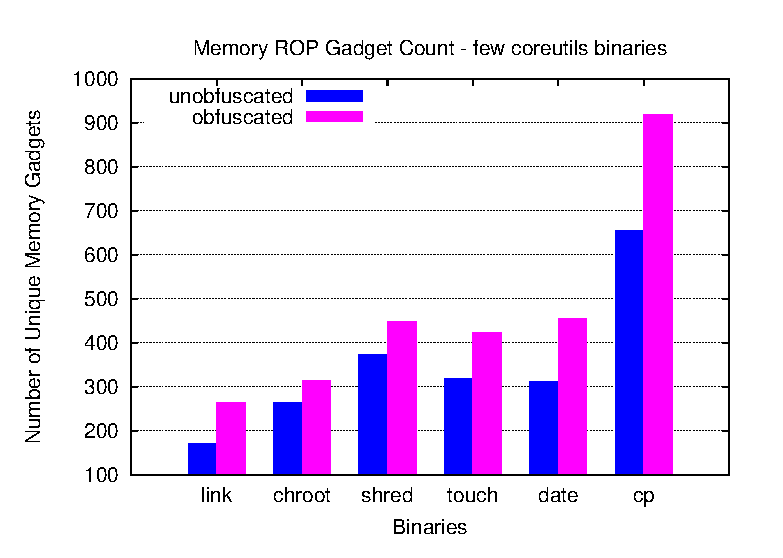
\includegraphics[width=\linewidth]{figures/memory.eps}
    \captionsetup{font=footnotesize, labelfont=bf, justification=centering}
    \caption{Memory gadget count for few `coreutils' binaries}
    \label{fig:memory}
\end{figure}

\begin{figure}[h]
    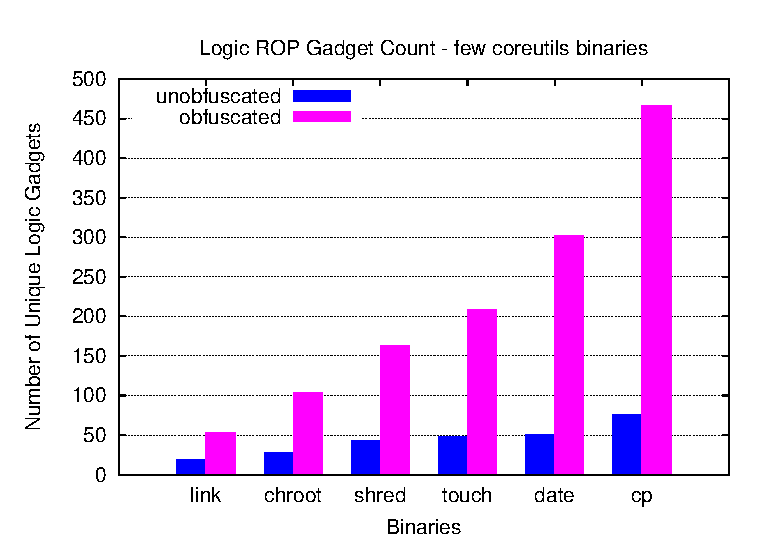
\includegraphics[width=\linewidth]{figures/logic.eps}
    \captionsetup{font=footnotesize, labelfont=bf, justification=centering}
    \caption{Logic gadget count for few `coreutils' binaries}
    \label{fig:logic}
\end{figure}


\begin{figure}[h]
    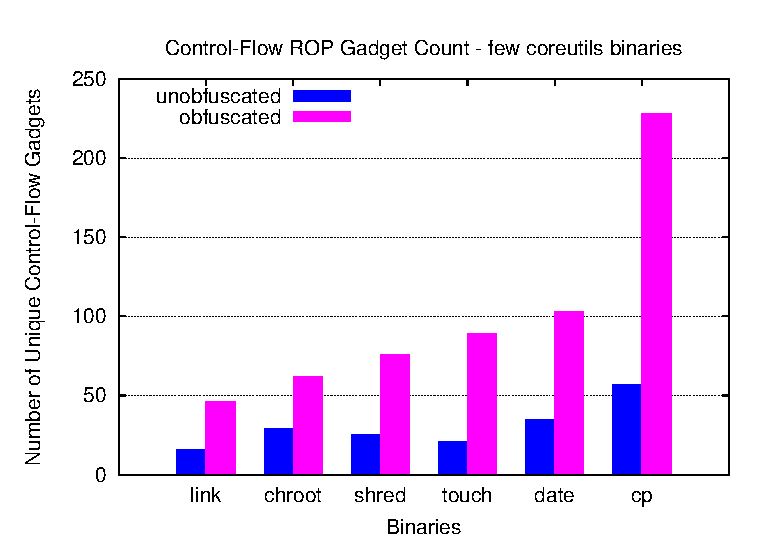
\includegraphics[width=\linewidth]{figures/control.eps}
    \captionsetup{font=footnotesize, labelfont=bf, justification=centering}
    \caption{Control-flow gadget count for few `coreutils' binaries}
    \label{fig:control}
\end{figure}


In addition to analyzing the number of gadgets, we looked at the actual 
gadgets for these binaries in order to do a qualitative analysis. We 
compared the gadgets found in each utility against their obfuscated 
binaries. There were some common gadgets between these binaries, usually 
at the lower memory address where the common preambles in ELF can be 
expected. However, the majority of the gadgets were very different in both 
sets of binaries and it was difficult to make any generalizations about 
them.


\subsection{Limitations and Future Work}
We discuss the limitations of our work here and also how it can be 
extended in future. 

\begin{itemize}
    \item We have selected our sample binaries for evaluation based on a 
    combination of ease of availability and security sensitivity. 
    Evaluation on binaries that are actually likely to be obfuscated would 
    have been more interesting. Such binaries, like DRM protection 
    software, are difficult to acquire in unobfuscated form since that 
    will completely defeat the purpose of obfuscation. 

    \item We have shown that for certain types of gadgets (logic, 
    control), obfuscation can significantly increase the number of gadgets 
    available. We have also shown that for small binaries, such increase 
    can potentially affect the feasibility of ROP attack. Due to the 
    limited time available to complete this project, we have not been able 
    to show that obfuscating a binary changes gadgets found from 
    non-Turing-complete to Turing-complete.

    \item It would be interesting if we can devise an actual attack on an 
    obfuscated binary and show that it is more difficult or impossible on 
    un-obfuscated binary. We have not attempted this, again due to limited 
    time.


    \item We have evaluated only one obfuscation tool, with limited set of 
    obfuscation transforms. It would be interesting to compare the results 
    we have obtained against other obfuscators. However, there are very 
    few open source or free obfuscators available for C, and they are 
    either rudimentary or old and not currently supported or maintained.
\end{itemize}
